\documentclass{../../oss-apphys-exam}

\begin{document}
%\genheader

\gentitle{1}{THERMODYNAMICS, PART 1}

\begin{questions}
  \classkickMCinstructions
  
  \question Air is made up primarily of nitrogen and oxygen. In an enclosed room
  with a constant temperature, which of the following statements is
  correct concerning the nitrogen and oxygen gases?
  \begin{choices}
    \choice The nitrogen gas molecules have a higher average kinetic energy than
    the oxygen gas molecules.
    \choice The nitrogen gas molecules have the same average kinetic energy as
    the oxygen gas molecules.
    \choice The nitrogen gas molecules have a lower average kinetic energy than
    the oxygen gas molecules.
    \choice More information is necessary to compare the average kinetic
    energies of the two gases.
  \end{choices}
  
  \question Air is made up primarily of nitrogen and oxygen. In an enclosed room
  with a constant temperature, which of the following statements is correct
  concerning the nitrogen and oxygen gases?
  \begin{choices}
    \choice The nitrogen gas molecules have a higher velocity than the oxygen
    gas molecules.
    \choice The nitrogen gas molecules have the same velocity as the oxygen gas
    molecules.
    \choice The nitrogen gas molecules have a lower velocity than the oxygen gas
    molecules.
    \choice It is impossible to compare the velocity of the two gases without
    knowing the temperature of the air and the percentage of nitrogen and
    oxygen in the room.
  \end{choices}
    
  \question When using the ideal gas law, $PV=nRT$,
  \begin{choices}
    \choice $P$ can be gauge pressure
    \choice $n$ can be in kilograms
    \choice $T$ can be in degrees Celsius
    \choice none of the above
  \end{choices}

  \question For ideal gases, the ratio $PV/T$ is
  \begin{choices}
    \choice equal to Avogadro's number
    \choice equal to Boltzmann's constant
    \choice independent of the number of molecules
    \choice independent of the chemical nature of the molecules
  \end{choices}

  \question The volume of an ideal gas at constant pressure is proportional to
  its
  \begin{choices}
    \choice Fahrenheit temperature
    \choice Celsius temperature
    \choice Absolute temperature
    \choice Molar mass
  \end{choices}


  \question Two identical rooms are connected by an open door. The temperature
  in one room is greater than the temperature in the other. Which room contains
  the most gas molecules?
  \begin{choices}
    \choice The warmer room.
    \choice The colder room.
    \choice The number of gas molecules will be the same in both rooms.
    \choice It is impossible to determine without more information.
  \end{choices}
  \newpage
  
  \question In an experiment, a gas is confined in a cylinder with a movable
  piston. Force is applied to the piston to increase the pressure and change the
  volume of the gas. Each time the gas is compressed, it is allowed to return
  to a room temperature of \SI{20}\celsius. The data gathered from the
  experiment is shown in the table. What should be plotted on the vertical and
  horizontal axes so the slope of the graph can be used to determine the number
  of moles of gas in the cylinder?
  \begin{center}
    \begin{tabular}{c|c}
      \textbf{Pressure} (\SI{e5}\pascal) &
      \textbf{Volume} (\SI{e-3}{\metre\cubed})
      \\ \hline\hline
      1.0 & 25 \\ \hline
      1.5 & 17 \\ \hline
      1.8 & 14 \\ \hline
      2.2 & 11 \\ \hline
      2.6 & 9.6\\ \hline
      3.3 & 7.6
    \end{tabular}
  \end{center}
  \begin{oneparchoices}
    \choice $P$ and $V^2$
    \choice $P$ and $V$
    \choice $P$ and $V^{1/2}$
    \choice $P$ and $1/V$
  \end{oneparchoices}

  %\uplevel{
  %  \cpic{.22}{mc-q17}
  %}
  %\question In an experiment, a sealed container with a volume of
  %\SI{100}{\milli\litre} is filled with hydrogen gas. The container is heated
  %to a variety of temperatures, and the pressure is measured. The data from the
  %experiment is plotted in the figure above. Which of the following methods can
  %be used to determine additional information regarding the gas? Select two
  %answers.
  %\begin{choices}
  %  \choice The slope can be used to calculate the number of atoms in the gas.
  %  \choice The area under the graph can be used to calculate the work done by
  %  the gas.
  %  \choice The vertical axis can be used to calculate the force the gas
  %  exerts on the container.
  %  \choice The $x$-intercept can be used to estimate the value of absolute
  %  zero.
  %\end{choices}
  
  \question Two sealed cylinders holding different gases are placed one on top
  of the other so heat can flow between them. Cylinder A is filled with
  hydrogen. Cylinder B is filled with helium moving with an average speed that
  is half that of the hydrogen atoms. Helium atoms have four times the mass of
  hydrogen atoms. Which of the following best describes the transfer of heat
  between the two containers by conduction?
  \begin{choices}
    \choice Net heat flows from cylinder A to cylinder B, because heat flows
    from higher kinetic energy atoms to lower kinetic energy atoms.
    \choice Net heat flows from cylinder B to cylinder A, because heat flows
    from higher kinetic energy atoms to lower kinetic energy atoms.
    \choice There is no net heat transfer between the two cylinders, because
    both gases have the same average atomic kinetic energy.
    \choice There is no net heat transfer between the two cylinders, because
    heat conduction requires the movement of atoms between the cylinder, and the
    cylinders are sealed.
  \end{choices}

  \uplevel{
    \cpic{.33}{mc-q26}
  }
  \question The graph above shows the distribution of speeds for one mole of
  hydrogen at temperature $T$, pressure $P$, and volume $V$. How would the
  graph change if the sample was changed from one mole hydrogen to one mole of
  argon at the same temperature, pressure, and volume?
  \begin{choices}
    \choice The peak will shift to the left
    \choice The peak will shift upward and to the left
    \choice The peak will shift to the right
    \choice The peak will shift downward and to the right
  \end{choices}
  \newpage
  
%  \question What is the volume of one mole of ideal gas at \SI{300}{\kelvin}
%  and at standard atmospheric pressure?
%  \begin{choices}
%    \choice\SI{23.2}\litre
%    \choice\SI{24.1}\litre
%    \choice\SI{24.6}\litre
%    \choice\SI{25.7}\litre
%  \end{choices}
  
  \question A fixed mass of oxygen (O\textsubscript{2}, molecular mass
  \SI{32}{\gram\per\mol}) is contained in a cylinder whose volume is 2.80
  litres. The pressure is \SI{148}{atm} when the temperature is
  \SI{23}\celsius. Find the mass of oxygen in the cylinder.
  \begin{choices}
    \choice\SI{20}\gram
    \choice\SI{80}\gram
    \choice\SI{140}\gram
    \choice\SI{280}\gram
    \choice\SI{546}\gram
  \end{choices}

  \classkickFRQinstructions
  
  %% THIS TAKEN FROM THE 2001 AP PHYSICS B EXAM FREE-RESPPONSE QUESTION #6
  %\uplevel{
  %  \centering
  %  \pic{.78}{gases}
  %  
  %  \underline{Note:} Figure not drawn to scale.
  %}
  %
  %\question A cylinder is fitted with a freely movable piston of area
  %\SI{1.20e-2}{\metre\squared} and negligible mass. The cylinder below the
  %piston is filled with a gas. At state 1, the gas has volume
  %\SI{1.50e-3}{\metre\cubed}, pressure \SI{1.02e5}\pascal, and the cylinder is
  %in contact with a water bath at a temperature of \SI0\celsius. The gas is
  %then taken through the following four-step process.
  %\begin{itemize}
  %\item A \SI{2.50}{\kilo\gram} metal block is placed on top of the piston,
  %  compressing the gas to State 2, with the gas still at \SI0\celsius.
  %\item The cylinder is then brought in contact with a boiling water bath,
  %  raising the gas temperature to \SI{100}{\celsius} at State 3.
  %\item The metal block is removed and the gas expands to State 4 still at
  %  \SI{100}\celsius.
  %\item Finally, the cylinder is again placed in contact with the water bath at
  %  \SI0\celsius, returning the system to State 1.
  %\end{itemize}
  %\begin{parts}
  %  \part Determine the pressure of the gas in State 2.
  %  \vspace{\stretch1}
  %  
  %  \part Determine the volume of the gas in State 2.
  %  \vspace{\stretch1}
  %  
  %  \part Indicate below whether the process from State 2 to State 3 is
  %  isothermal, isobaric, or adiabatic. Explain your reasoning.
  %
  %  \vspace{.1in}
  %  \underline{\hspace{.3in}} Isothermal\hspace{.5in}
  %  \underline{\hspace{.3in}} Isobaric\hspace{.5in}
  %  \underline{\hspace{.3in}} Adiabatic
  %  \vspace{\stretch1}
  %      
  %  \part Is the process from state 4 to state 1 isobaric? Explain your
  %  reasoning.
  %
  %  \vspace{.1in}\underline{\hspace{.3in}}Yes\hspace{.5in}
  %  \underline{\hspace{.3in}} No
  %  \vspace{\stretch1}
  %
  %  \part Determine the volume of the gas in state 4.
  %  \vspace{\stretch1}
  %\end{parts}
  %\newpage


  
  \question The specific heat capacity of air at \SI0{\celsius} is
  \SI{1.00}{\joule\per\gram.\kelvin} measured at constant pressure. Assuming
  that air is an ideal gas with a molar mass of $M=\SI{29}{\gram\per\mol}$,
  \begin{parts}
    \part what is its specific heat capacity at \SI0{\celsius} at constant
    volume?
    \vspace{\stretch1}
    
    \part How much internal energy is there in 1 L of air at \SI0\celsius?
    \vspace{\stretch1}
  \end{parts}

  \question One mole of a ideal diatomic gas is heated at constant volume from
  300 to \SI{600}\kelvin.
  \begin{parts}
    \part Find the increase in internal energy, work done, and heat added
    \vspace{\stretch1}
    
    \part Find the same quantities if the gas is heated at constant pressure.
    (Use the first law of thermodynamic.)% and your results in part (a) to
    %calculate the work done.)
    %\vspace{\stretch1}
    %
    %\part Calculate the work done in part (b) directly using the definition of
    %work.
    \vspace{\stretch1}
  \end{parts}
  \newpage


  \question A piece of ice is dropped from a height $H$.
  \begin{parts}
    \part Find the minimum value of $H$ such that all the ice melts when it
    makes a completely inelastic collision with the ground. Assume that all
    the mechanical energy lost goes into melting the ice.
    \vspace{\stretch1}

    \part Is it reasonable to neglect the variation in the acceleration of
    gravity in doing this problem
    \vspace{\stretch1}

    \part Comment on the reasonableness of neglecting air resistance (drag).
    What effect would air resistance have on your answer to part (a)?
    \vspace{\stretch1}
  \end{parts}

  \question A \SI{450}{\milli\litre} cup of coffee is too hot to drink at
  \SI{91}\celsius, so \SI{100}{\milli\litre} of cold water at
  \SI{6.5}{\celsius} is added to cool it off.
  \begin{parts}
    \part What is the final temperature of the drink?
    \vspace{\stretch2}
    \part What assumptions do you have to make in order to solve this problem?
    \vspace{\stretch1}
  \end{parts}
  \newpage
  
  
  % THIS TAKEN FROM THE 2005 AP PHYSICS B EXAM FREE-RESPPONSE QUESTION #6
  \uplevel{
    \centering
    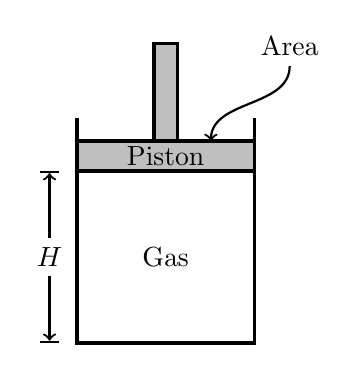
\begin{tikzpicture}[yscale=.95]
      \begin{scope}[very thick]
        \draw (0,3)--(0,0)--(2.25,0)--(2.25,3);
        \draw[fill=lightgray] (0,2.3) rectangle(2.25,2.7) node[midway]{Piston};
        \draw[fill=lightgray] (2.25/2-.15,2.7) rectangle (2.25/2+.15,4);
      \end{scope}
      \draw[thick,|<->|] (-.35,0)--(-.35,2.3) node[midway,fill=white]{$H$};
      \draw[thick,<-] (1.7,2.7) to[out=90,in=270] (2.7,3.7) node[above]{Area};
      \node at (2.25/2,2.3/2) {Gas};
    \end{tikzpicture}
  }
  
  \question An experiment is performed to determine the number $n$ of moles of
  an ideal gas in the cylinder shown above. The cylinder is fitted with a
  movable, frictionless piston of area $A$. The piston is in equilibrium and is
  supported by the pressure of the gas. The gas is heated while its pressure
  $P$ remains constant. Measurements are made of the temperature $T$ of the gas
  and the height $H$ of the bottom of the piston above the base of the cylinder
  and are recorded in the table below. Assume that the thermal expansion of the
  apparatus can be ignored.
  \begin{center}
    \begin{tabular}{|c|c|}
      \hline
      $T$ (\si\kelvin) & $H$ (\si\metre) \\ \hline\hline
      300 & 1.11 \\
      325 & 1.19 \\
      355 & 1.29 \\
      375 & 1.37 \\
      405 & 1.47 \\
      \hline
    \end{tabular}
  \end{center}
  \begin{parts}
    \part Write a relationship between the quantities $T$ and $H$, in terms of
    the given quantities and fundamental constants, that will allow you to
    determine $n$.
    \vspace{\stretch1}
    
    \part Plot the data on the axes below so that you will be able to determine
    $n$ from the relationship in part (a). Label the axes with appropriate
    numbers to show the scale.
    \begin{center}
      \begin{tikzpicture}[scale=.5]
        \draw[help lines,gray] grid (15,11);
        \draw[axes] (0,0)--(16,0) node[right]{$T$ (\si\kelvin)};
        \draw[axes] (0,0)--(0,12) node[above]{$H$ (\si\metre)};
      \end{tikzpicture}
    \end{center}
    
    \part Using your graph and the values $A=\SI{.027}{\metre\squared}$ and
    $P=\SI{1.0}{atm}$, determine the experimental value of $n$.
    \vspace{\stretch1}
  \end{parts}
\end{questions}
\end{document}
